
\section{Building process}
As seen from Figure \ref{Fig:Build_process}, the building process is composed by various phases:
\begin{itemize}
	\item Using an editor, you create the source and header files.
	\item The makefile defines which operations are needed to complete the build and which files have to be build.
	\item The preprocessor analyzes the source code and runs the preprocessor directives: macros, \#defines, ecc.. are expanded in "normal code": the full source is now ready to be compiled and goes in one *.i file. This operation can be seen by stopping the building process with the command \code{g++ -E main.c -o hello.i}
	\item After compiling the *.i files we get the assembly code, another human-readable text file. This output file can be seen by stopping the building process with the command \code{g++ -c hello.c}
	\item The next step is assembling the code: an *.o (object) file is generated, that's something really close the machine code, but still not hardware dependent: the memory addresses are still relative and the library calls are still not included.
	\item The final step is linking: it adds the static libraries to the code and generates the final executable file.
\end{itemize}
\begin{figure}[h]
	\centering
	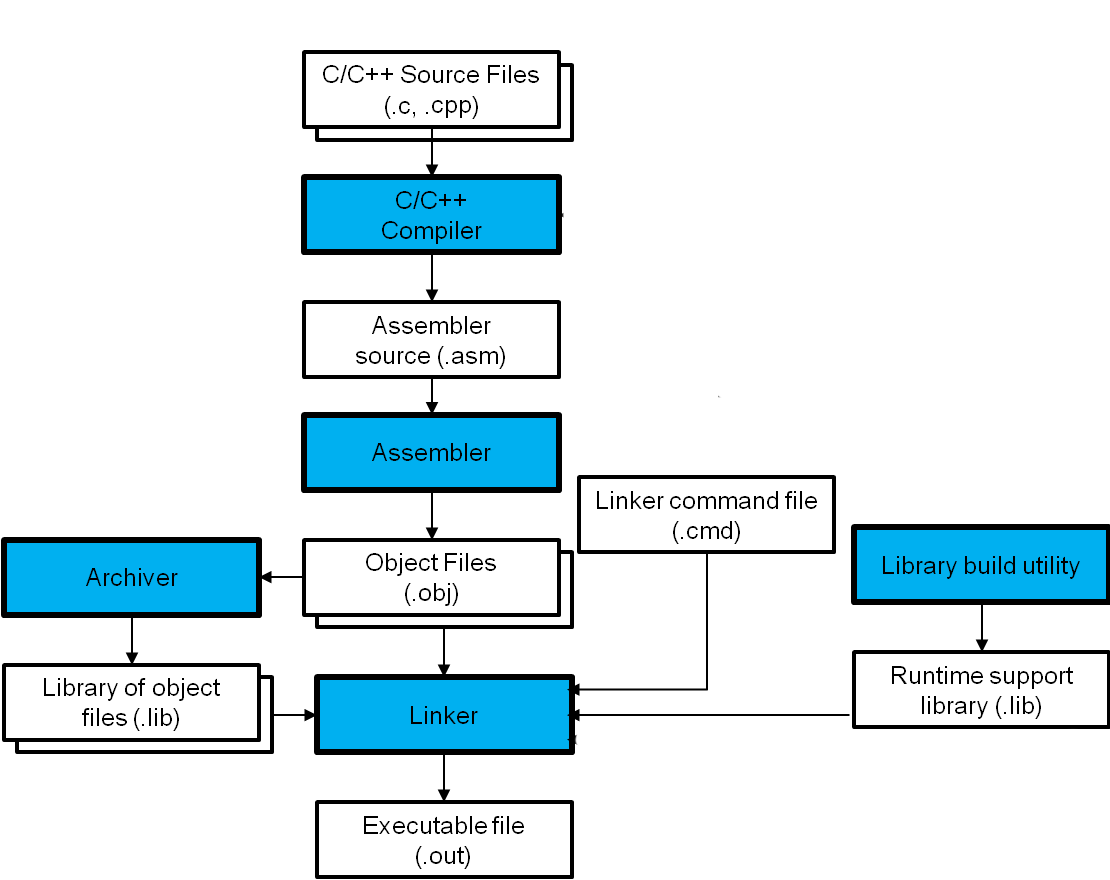
\includegraphics[width=\textwidth]{gfx/build_process}
	
	\caption{Build Process Procedure}
	\label{Fig:Build_process}
\end{figure}

\section{Makefile}
TODO

\section{Linker Script}
The linker script is a file that defines where the various parts of the compiled code are actually stored in memory.

The simplest possible linker script has just one command:\code[SECTIONS]. This command describes the memory layout of the building output file.

Let's assume that the program consists only of code, initialized data and uninitialized data: these will be, respectively, stored in the \code[.text], \code{.data} and \code{.bss} sections.

The linker script that could place these section in the correct parts of the memory would be something like:

\begin{lstlisting}
SECTIONS
{
	. = 0X10000; /* everything starts at this address*/
	.text : {*(.text)} /*every text file goes here*/ 
	. = 0x8000000;
	.data : { *(.data)}
	.bss : {*.(.bss)}

}

\end{lstlisting}


%\begin{figure}[h]
%	\centering
%	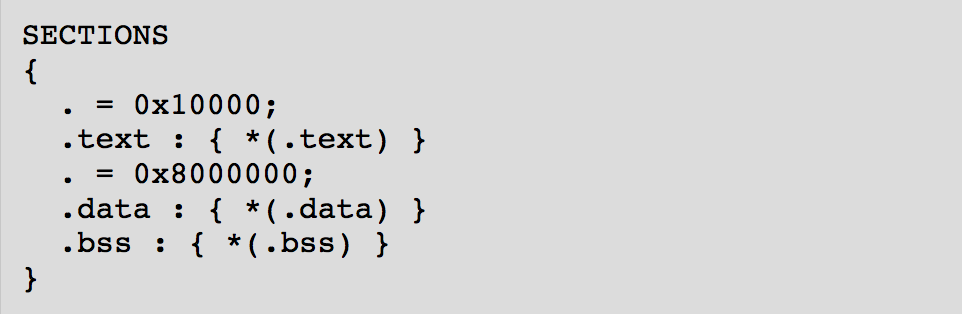
\includegraphics[width=\textwidth/3]{gfx/linker_file}
%	
%	\caption{Linker file example}
%	\label{Fig:Linker File}
%\end{figure}

